\section{Вынужденное движение}
\subsection{Линейная система}
Вернемся к системе, рассмотренной в прошлой лабораторной работе:
\begin{equation}
    \ddot{y} + a_1 \dot{y} + a_0 y = u
    \label{eq:system}
\end{equation}
структурная схема приведена на рисунке \ref{fig:scheme1}.
\begin{figure}[ht!]
    \centering
    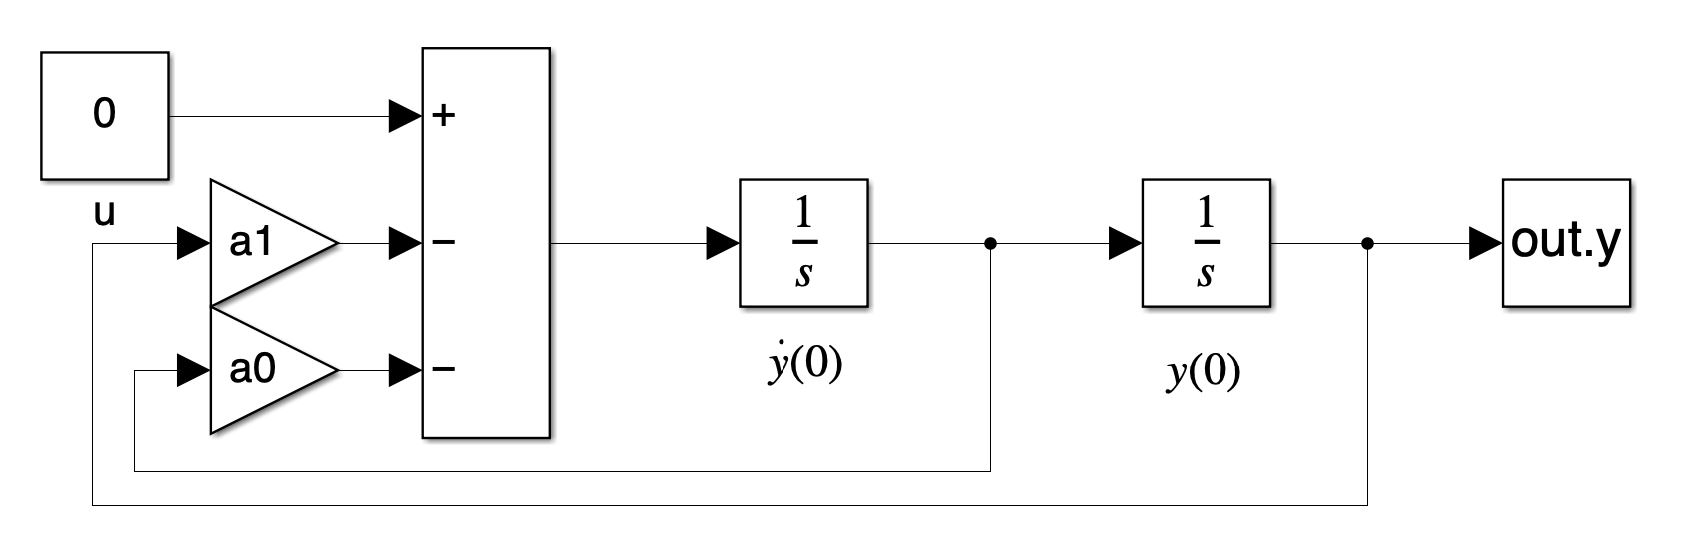
\includegraphics[width=\textwidth]{media/scheme1.png}
    \caption{Структурная схема системы}
    \label{fig:scheme1}
\end{figure}

\subsection{Моделирование при различных входных воздействиях}
Рассмотрим поведение данной системы при параметрах $a_0$, $a_1 = 1$, 
ранее полученных из корней характеристического уравнения: 
\begin{table}[ht!]
    \centering
    \begin{tabular}{|c|c|c|c|c|c|c|c|c|}
        \hline
        Номер & $\lambda_1$ & $\lambda_2$ & $a_0$ & $a_1$ \\
        \hline
        $1$ & $-2.8 + 6j$ & $-2.8 - 6j$ & $43.84$ & $5.6$ \\
        \hline
        $2$ & $18j$ & $-18j$ & $324$ & $0$ \\
        \hline
        $3$ & $0.8 + 6j$ & $0.8 - 6j$ & $36.64$ &  $-1.6$ \\
        \hline
    \end{tabular}
    \caption{Начальные условия и коэффициенты}
    \label{tab:initial_conditions}
\end{table}
Начальными условиями для системы будут:
\begin{table}[ht!]
    \centering
    \begin{tabular}{|c|c|c|}
        \hline 
        Номер & $y(0)$ & $\dot{y}(0)$ \\
        \hline
        $1$ & $-1$ & $0$ \\
        \hline
        $2$ & $0$ & $0$ \\
        \hline
        $3$ & $1$ & $0$ \\
        \hline
    \end{tabular}
    \caption{Начальные условия}
\end{table}

В качестве внешнего воздействия $u(t)$ возьмем следующие функции:
\begin{equation}
    u_1(t) = 0.5\quad u_2(t) = 0.5t\quad u_3(t) = \cos(2t)
\end{equation}

Промоделируем системы. Для каждого набора коэффициентов и входных сигналов промоделируем 
систему при различных входных воздействиях (см. рис \ref{fig:case1_input1} - \ref{fig:case_3_input_3}).
\begin{figure}[ht!]
    \centering
    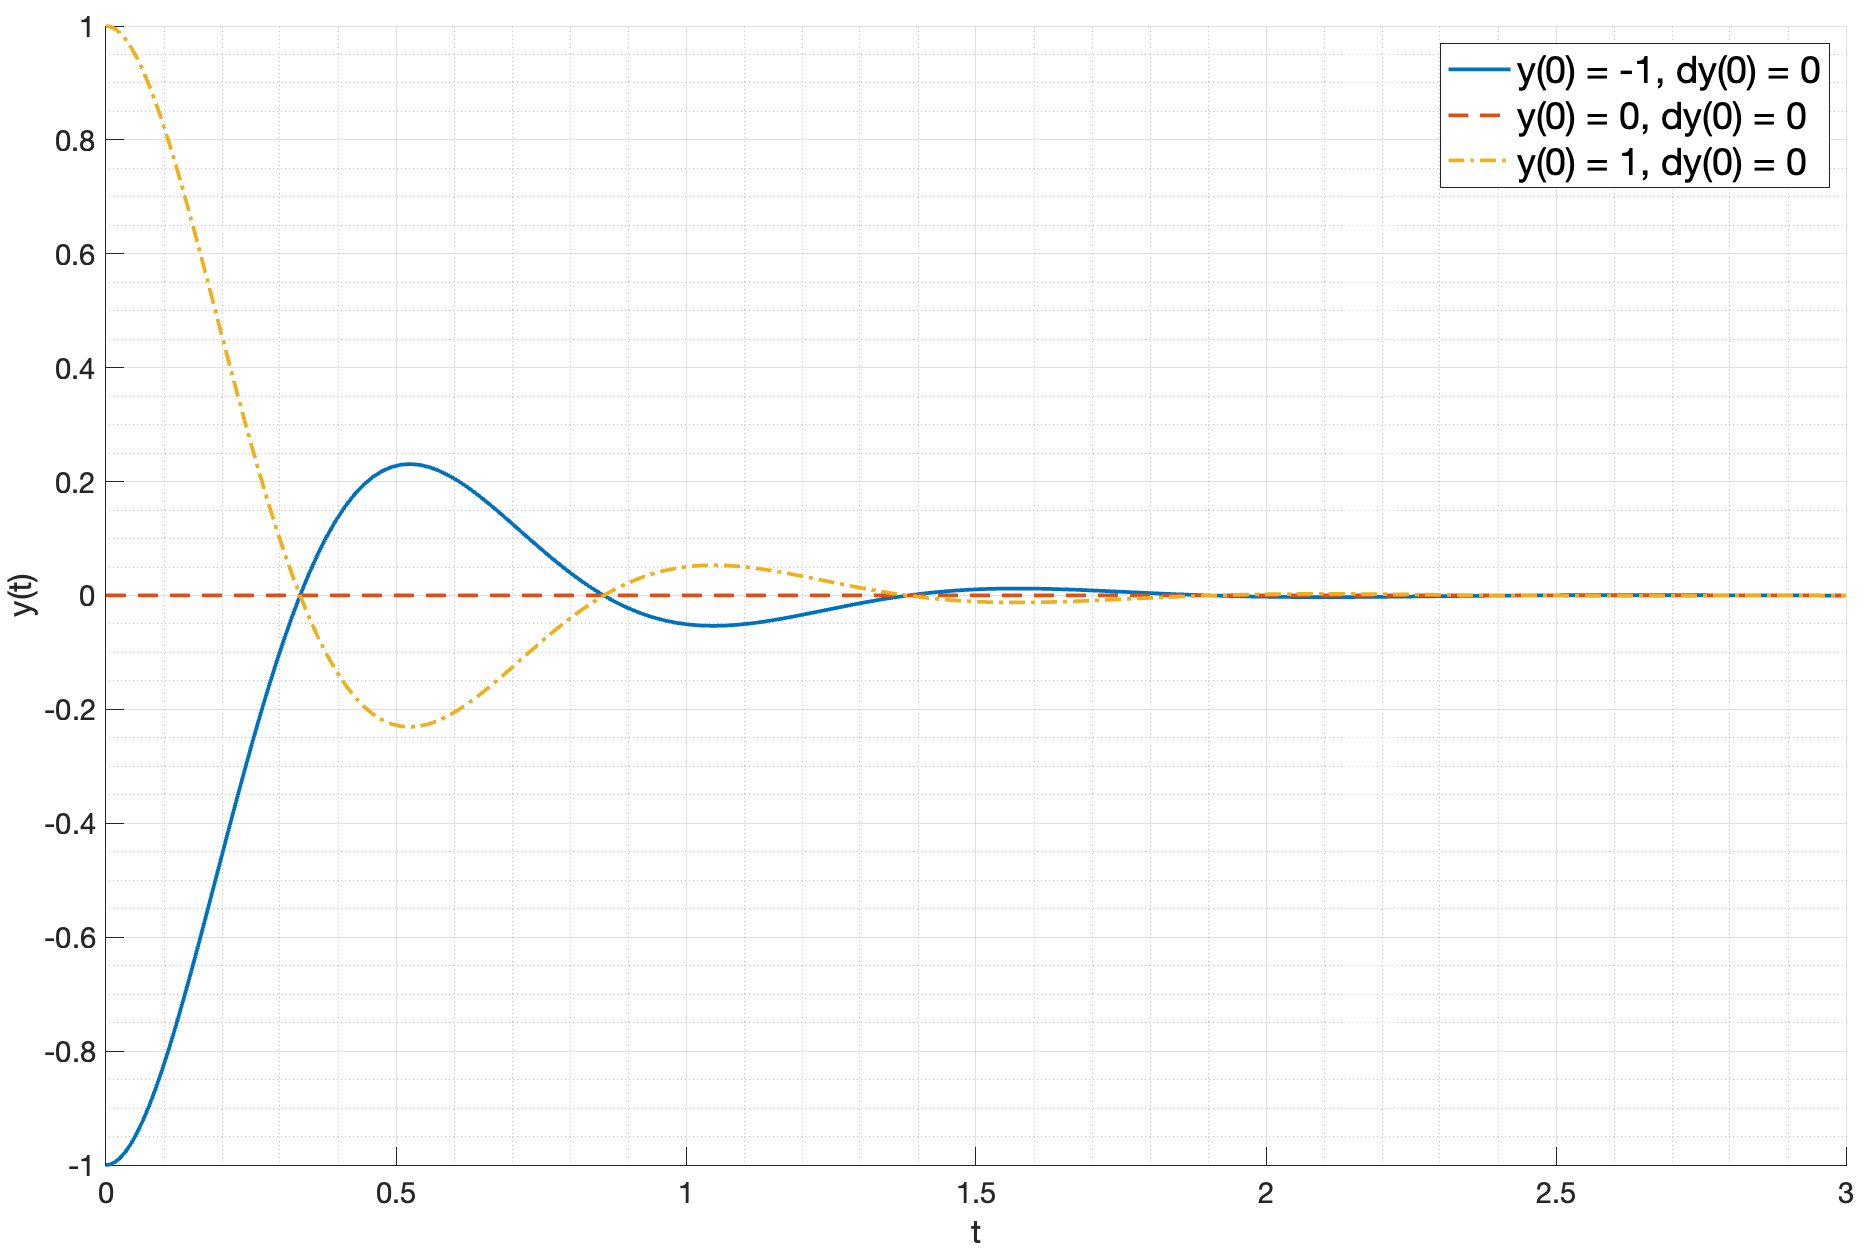
\includegraphics[width=\textwidth]{media/plots/case1_input1.png}
    \caption{$a_0 = 43.84, a_1 = 5.6, u(t) = 0.5$}
    \label{fig:case1_input1}
\end{figure}
\begin{figure}[ht!]
    \centering
    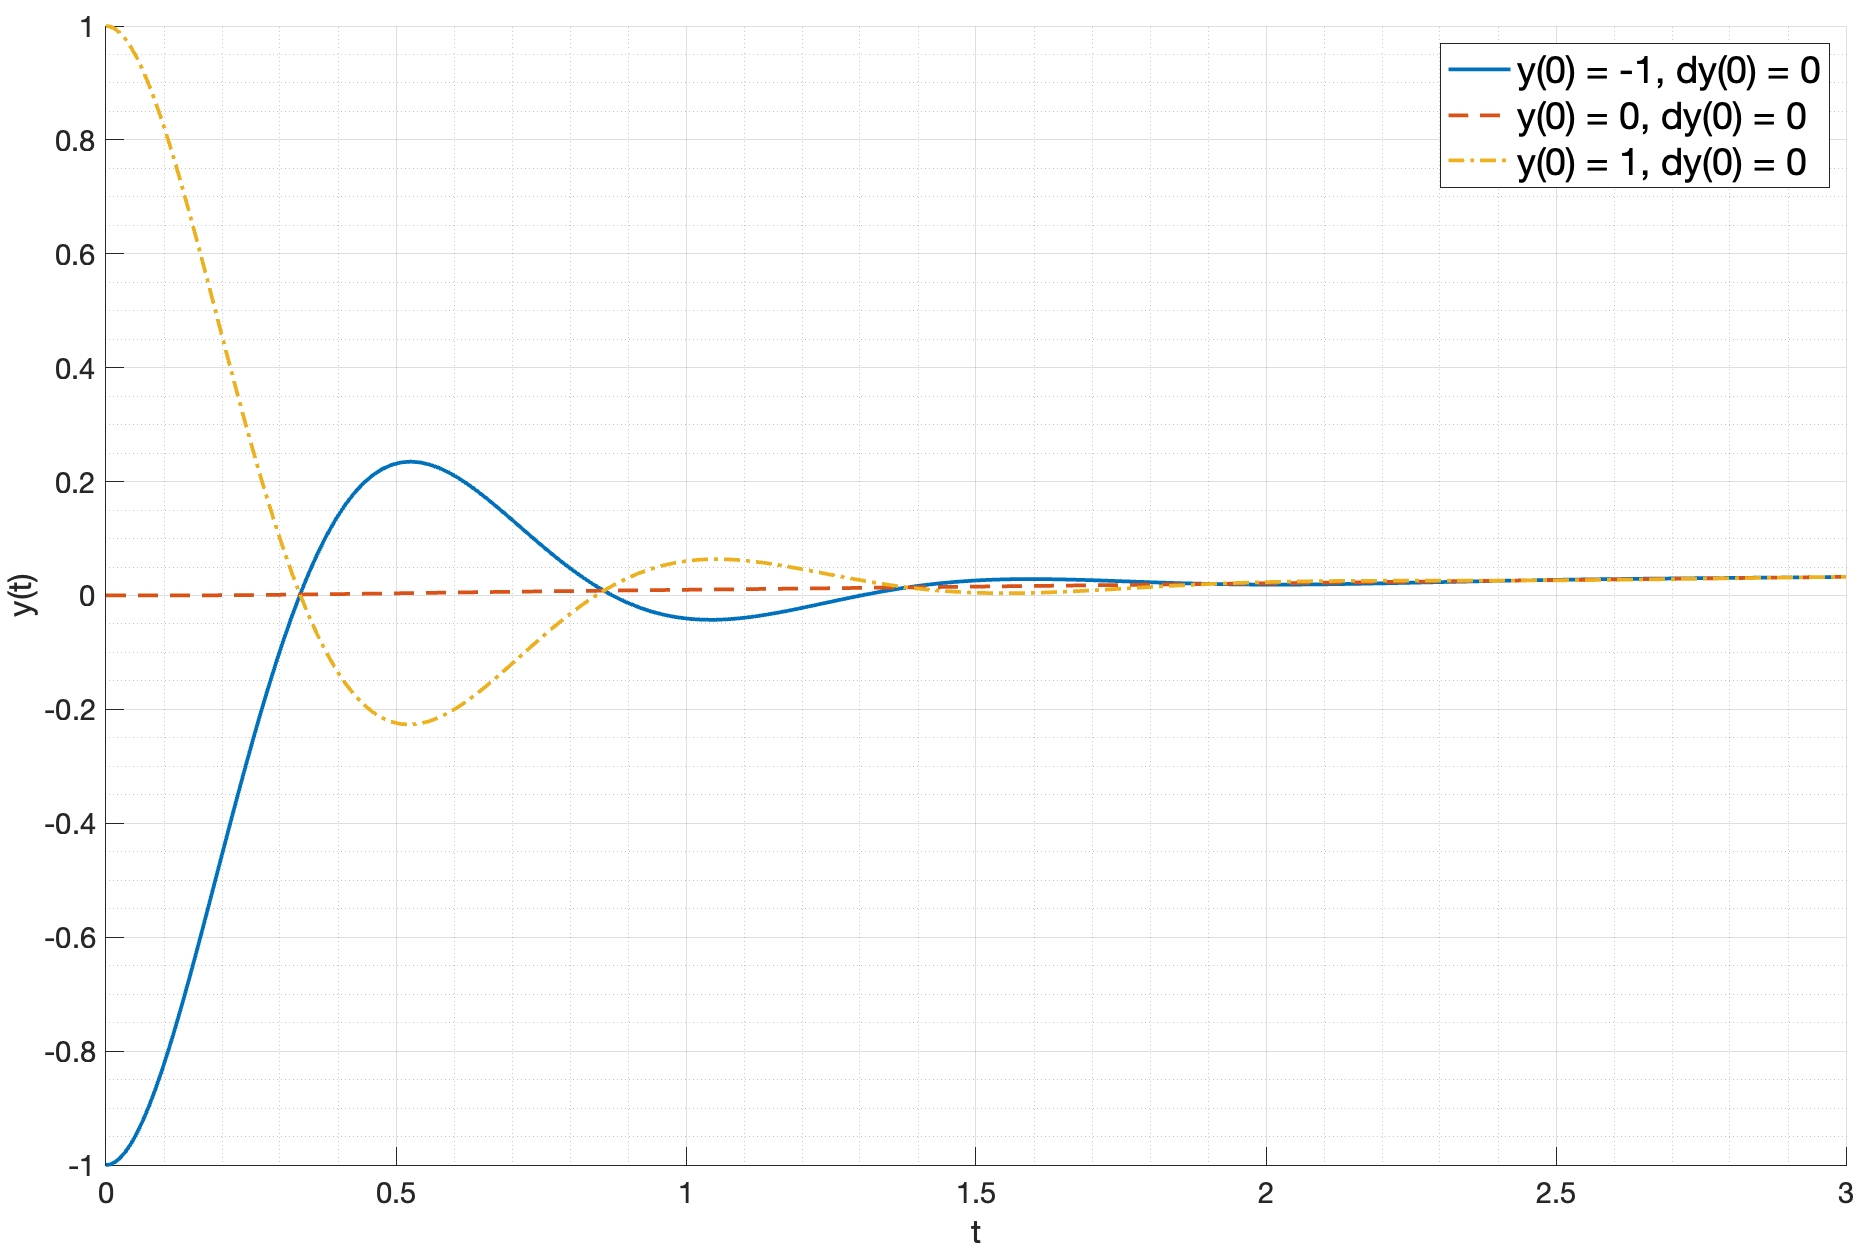
\includegraphics[width=\textwidth]{media/plots/case1_input2.png}
    \caption{$a_0 = 43.84, a_1 = 5.6, u(t) = 0.5t$}
    \label{fig:case1_input2}
\end{figure}
\begin{figure}[ht!]
    \centering
    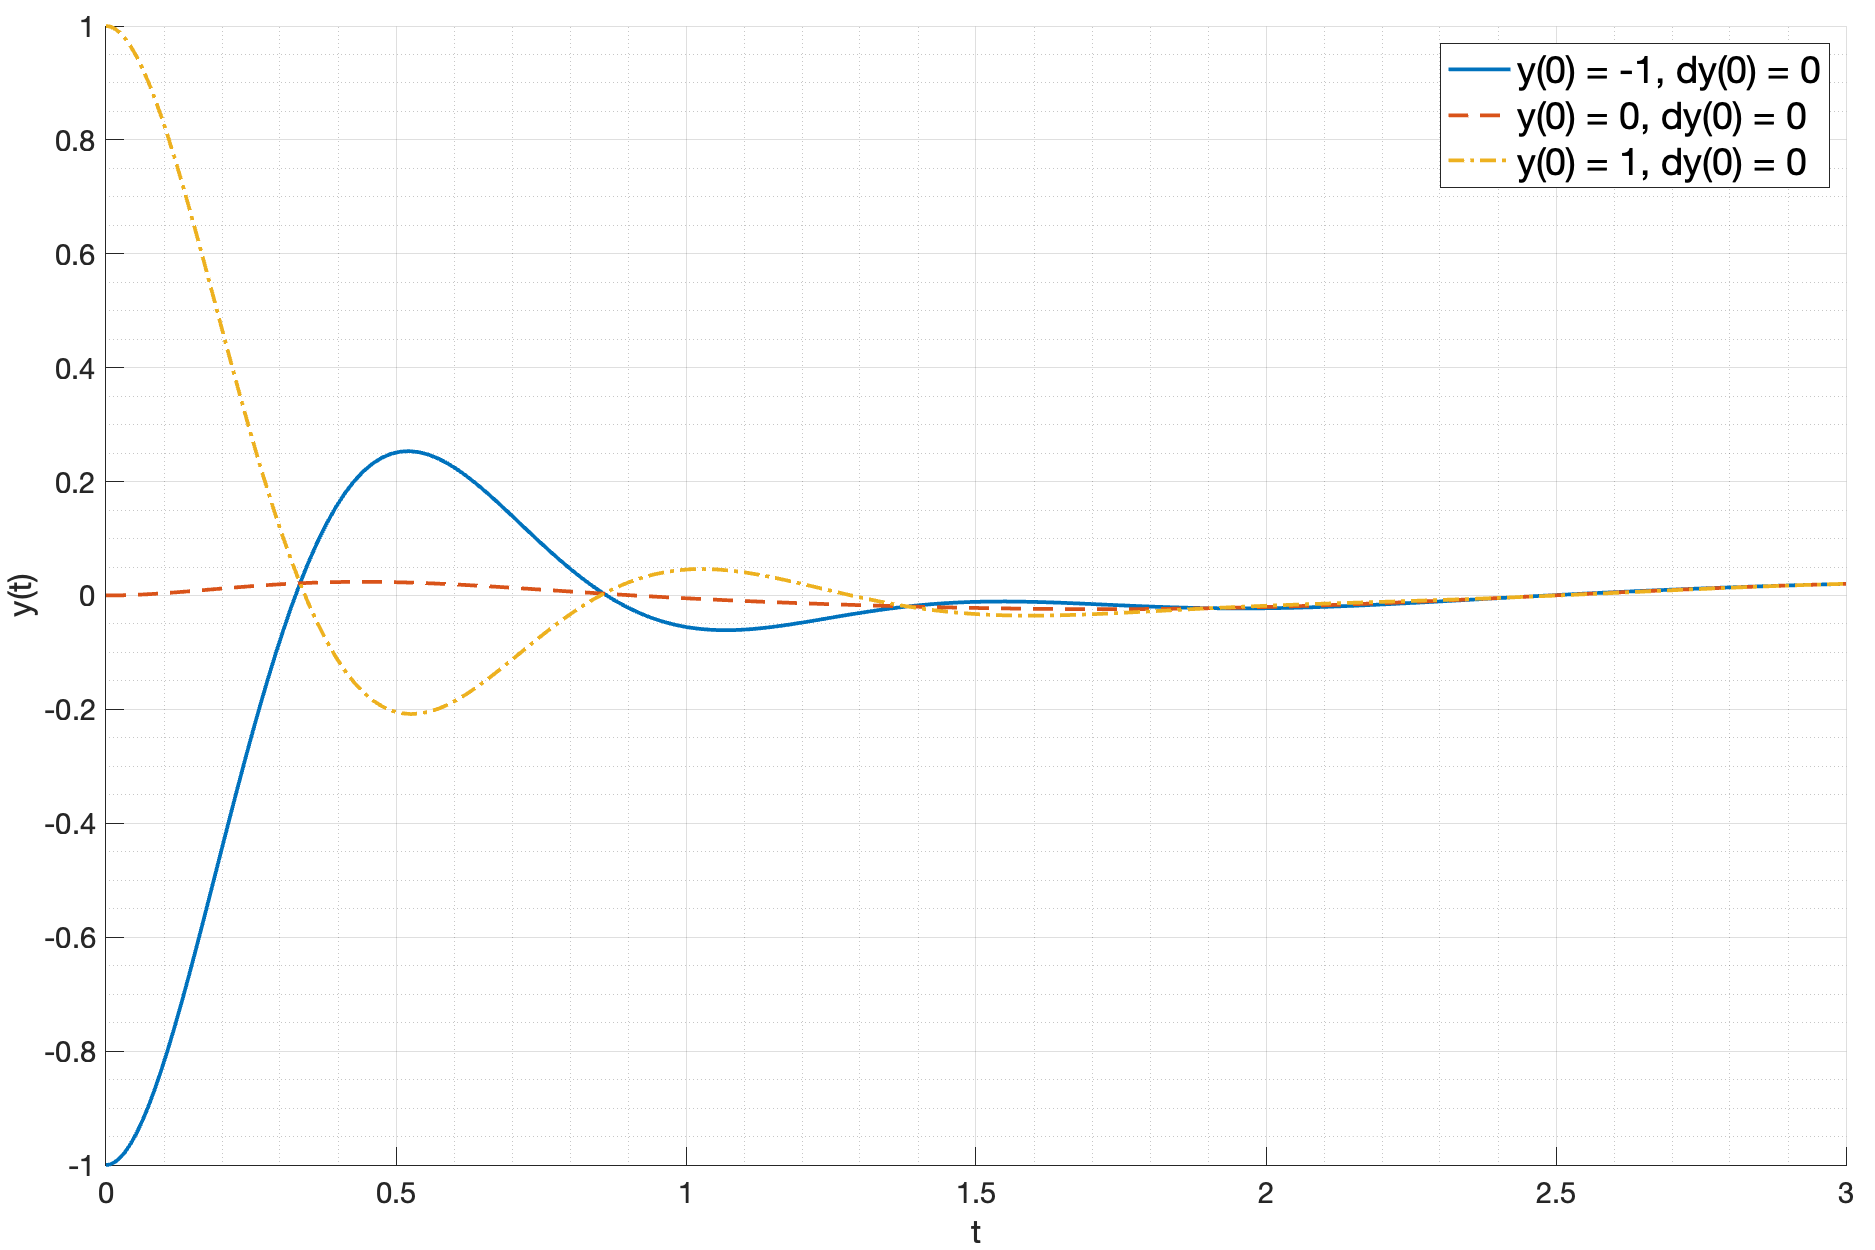
\includegraphics[width=\textwidth]{media/plots/case1_input3.png}
    \caption{$a_0 = 43.84, a_1 = 5.6, u(t) = \cos(2t)$}
    \label{fig:case1_input3}
\end{figure}

\begin{figure}[ht!]
    \centering
    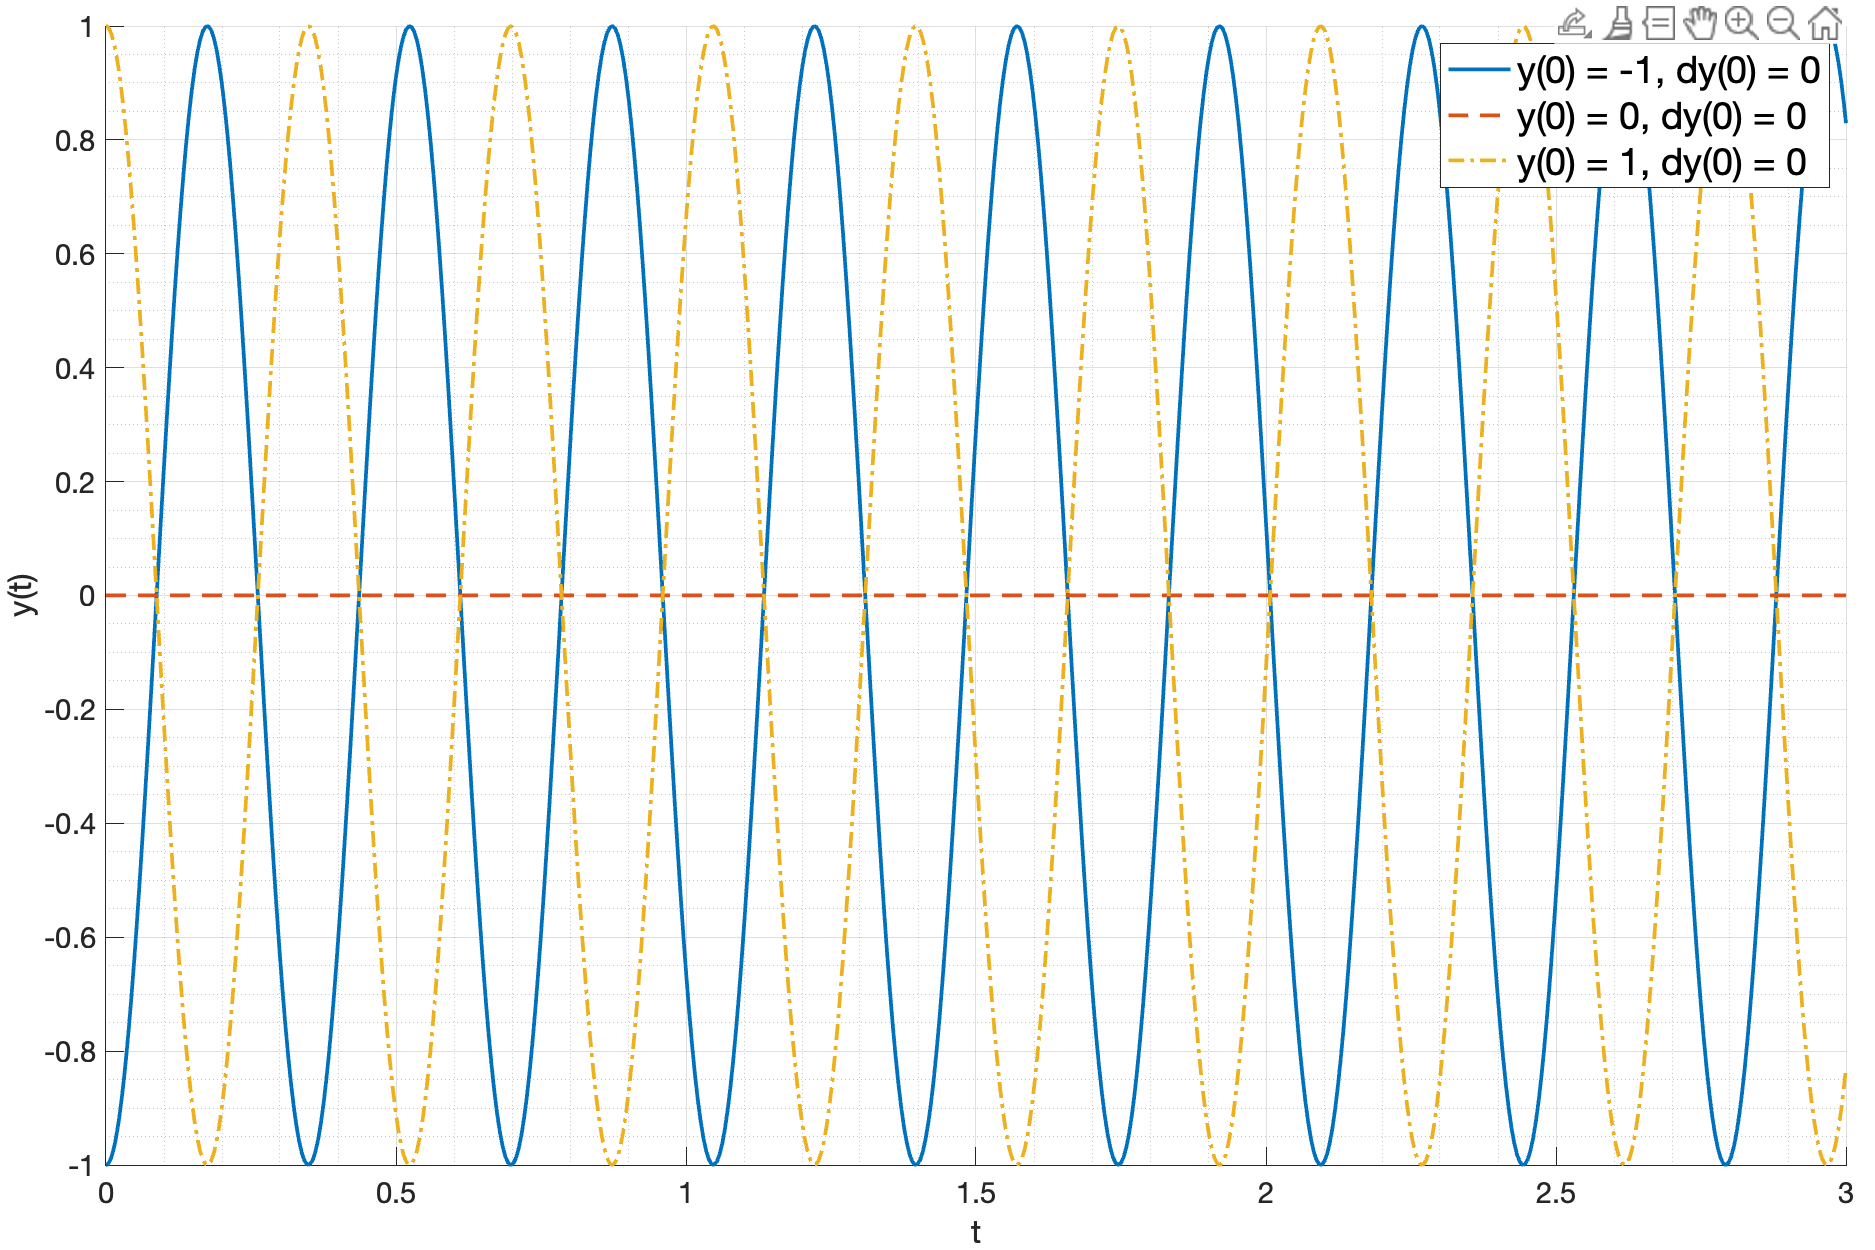
\includegraphics[width=\textwidth]{media/plots/case2_input1.png}
    \caption{$a_0 = 324, a_1 = 0, u(t) = 0.5$}
    \label{fig:case2_input1}
\end{figure}
\begin{figure}[ht!]
    \centering
    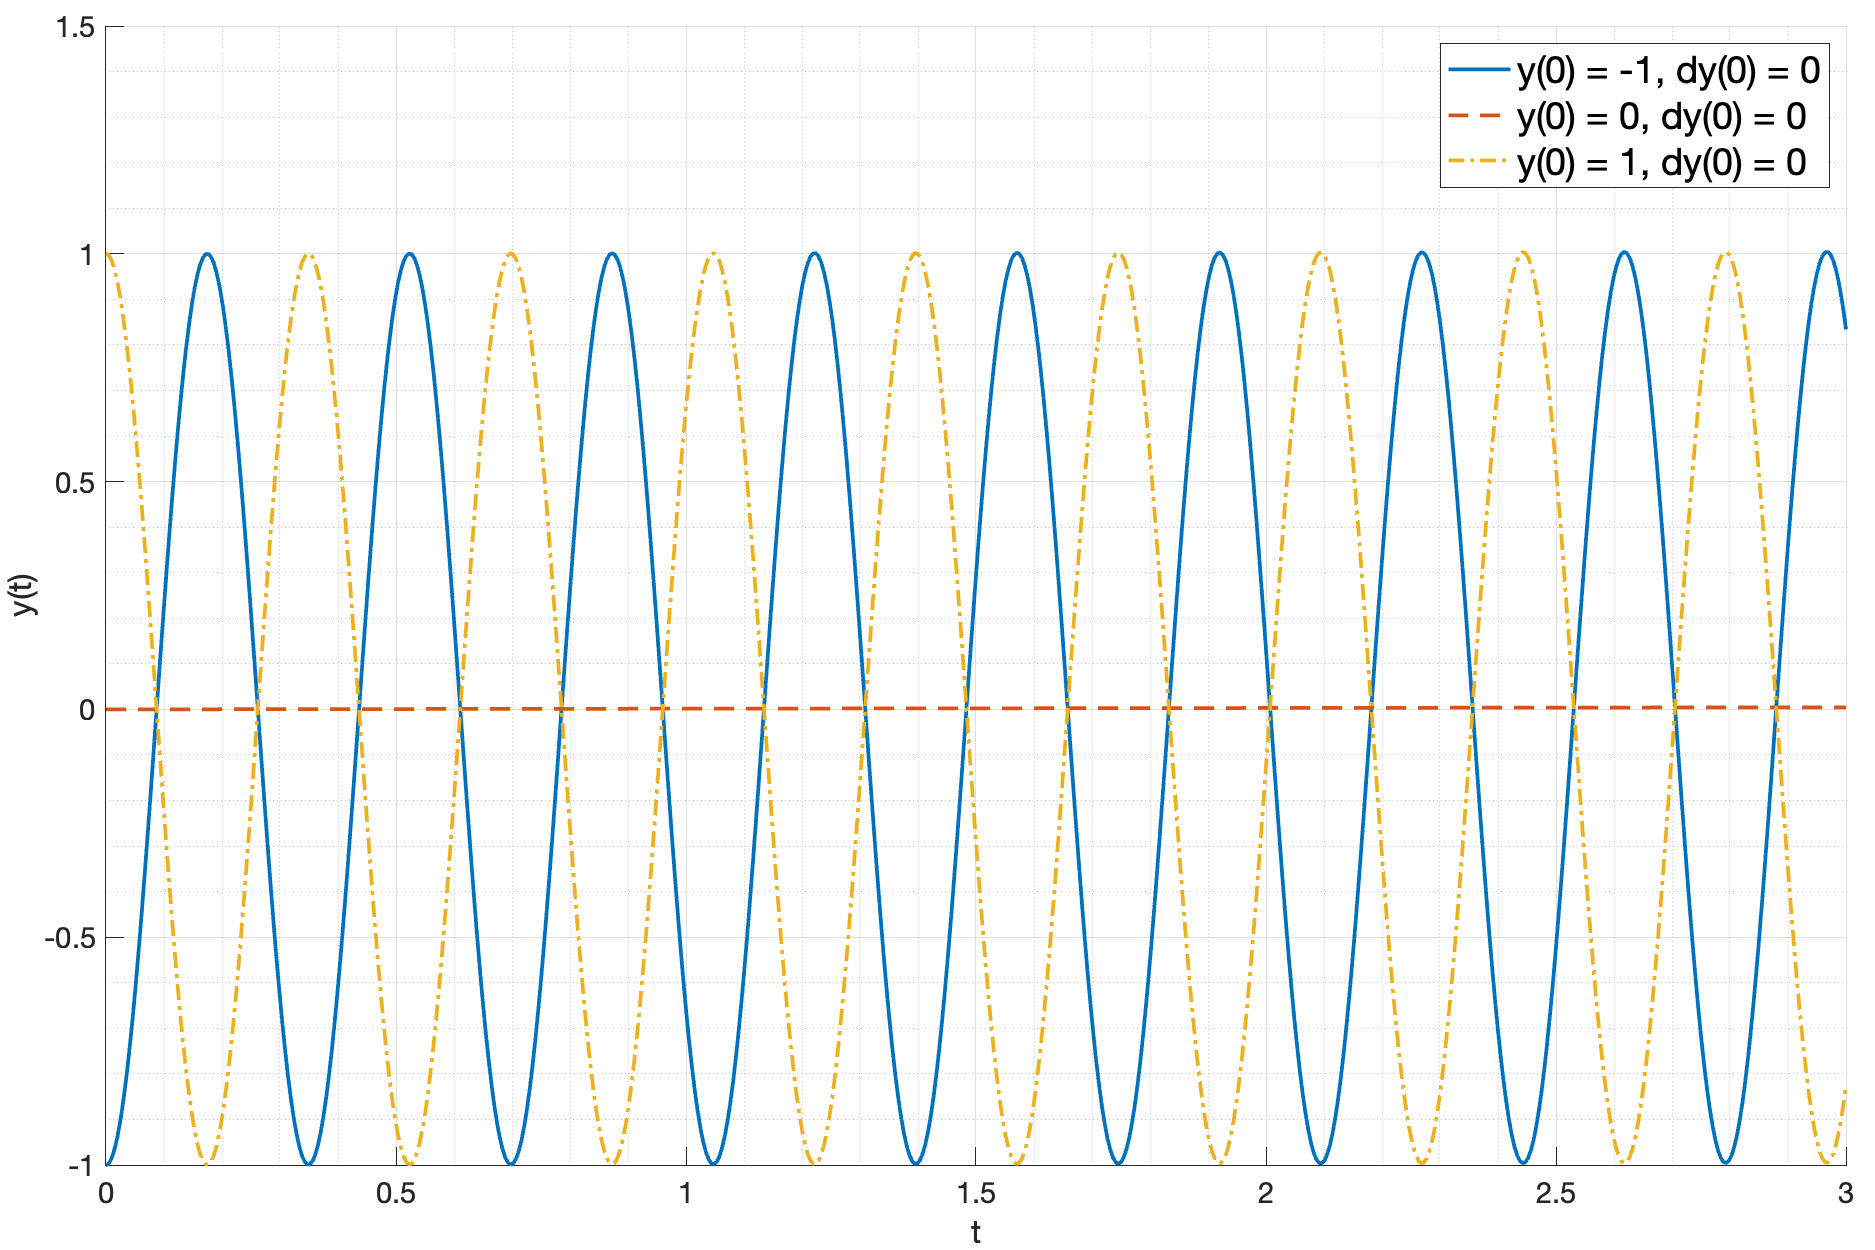
\includegraphics[width=\textwidth]{media/plots/case2_input2.png}
    \caption{$a_0 = 324, a_1 = 0, u(t) = 0.5t$}
    \label{fig:case2_input2}
\end{figure}
\begin{figure}[ht!]
    \centering
    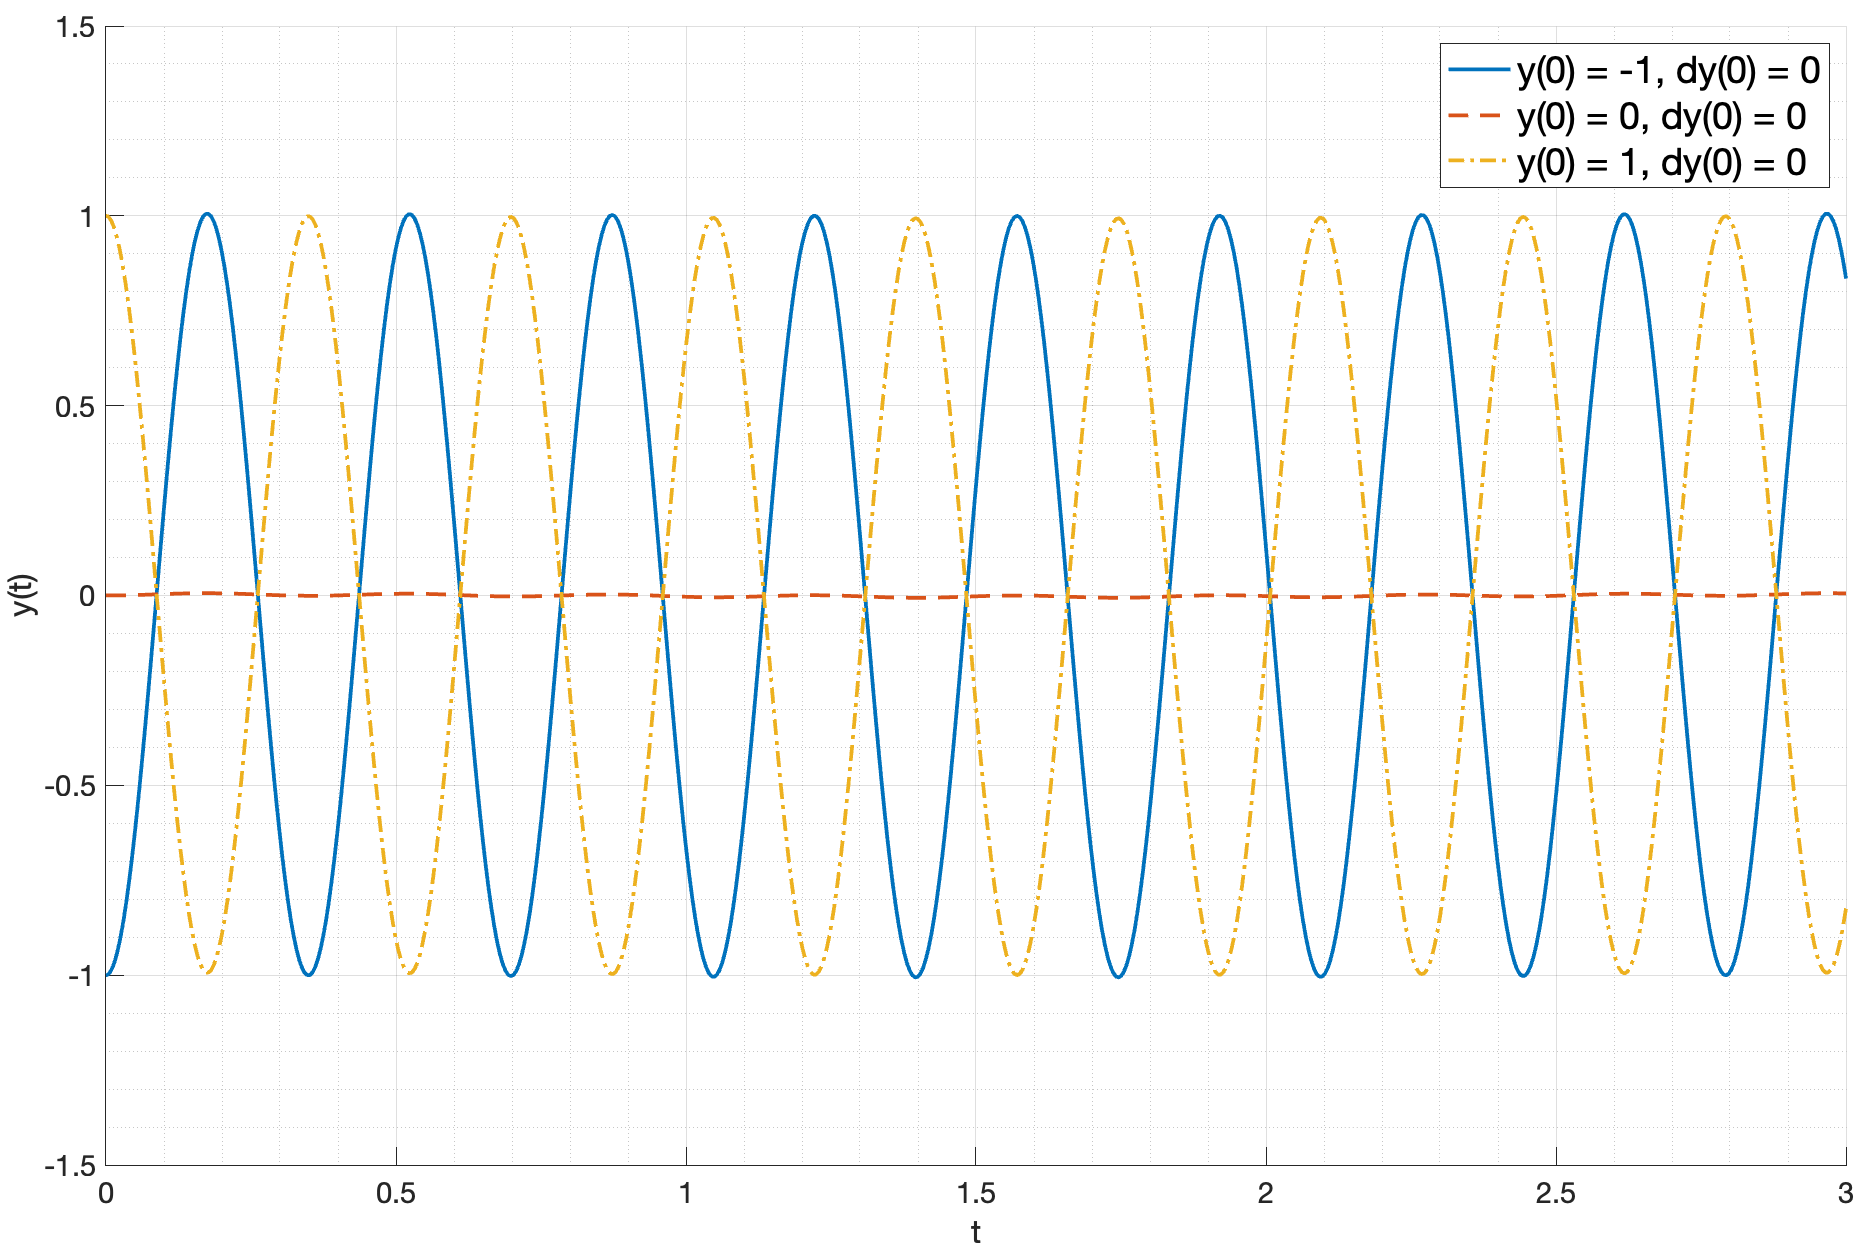
\includegraphics[width=\textwidth]{media/plots/case2_input3.png}
    \caption{$a_0 = 324, a_1 = 0, u(t) = \cos(2t)$}
    \label{fig:case2_input3}
\end{figure}

\begin{figure}[ht!]
    \centering
    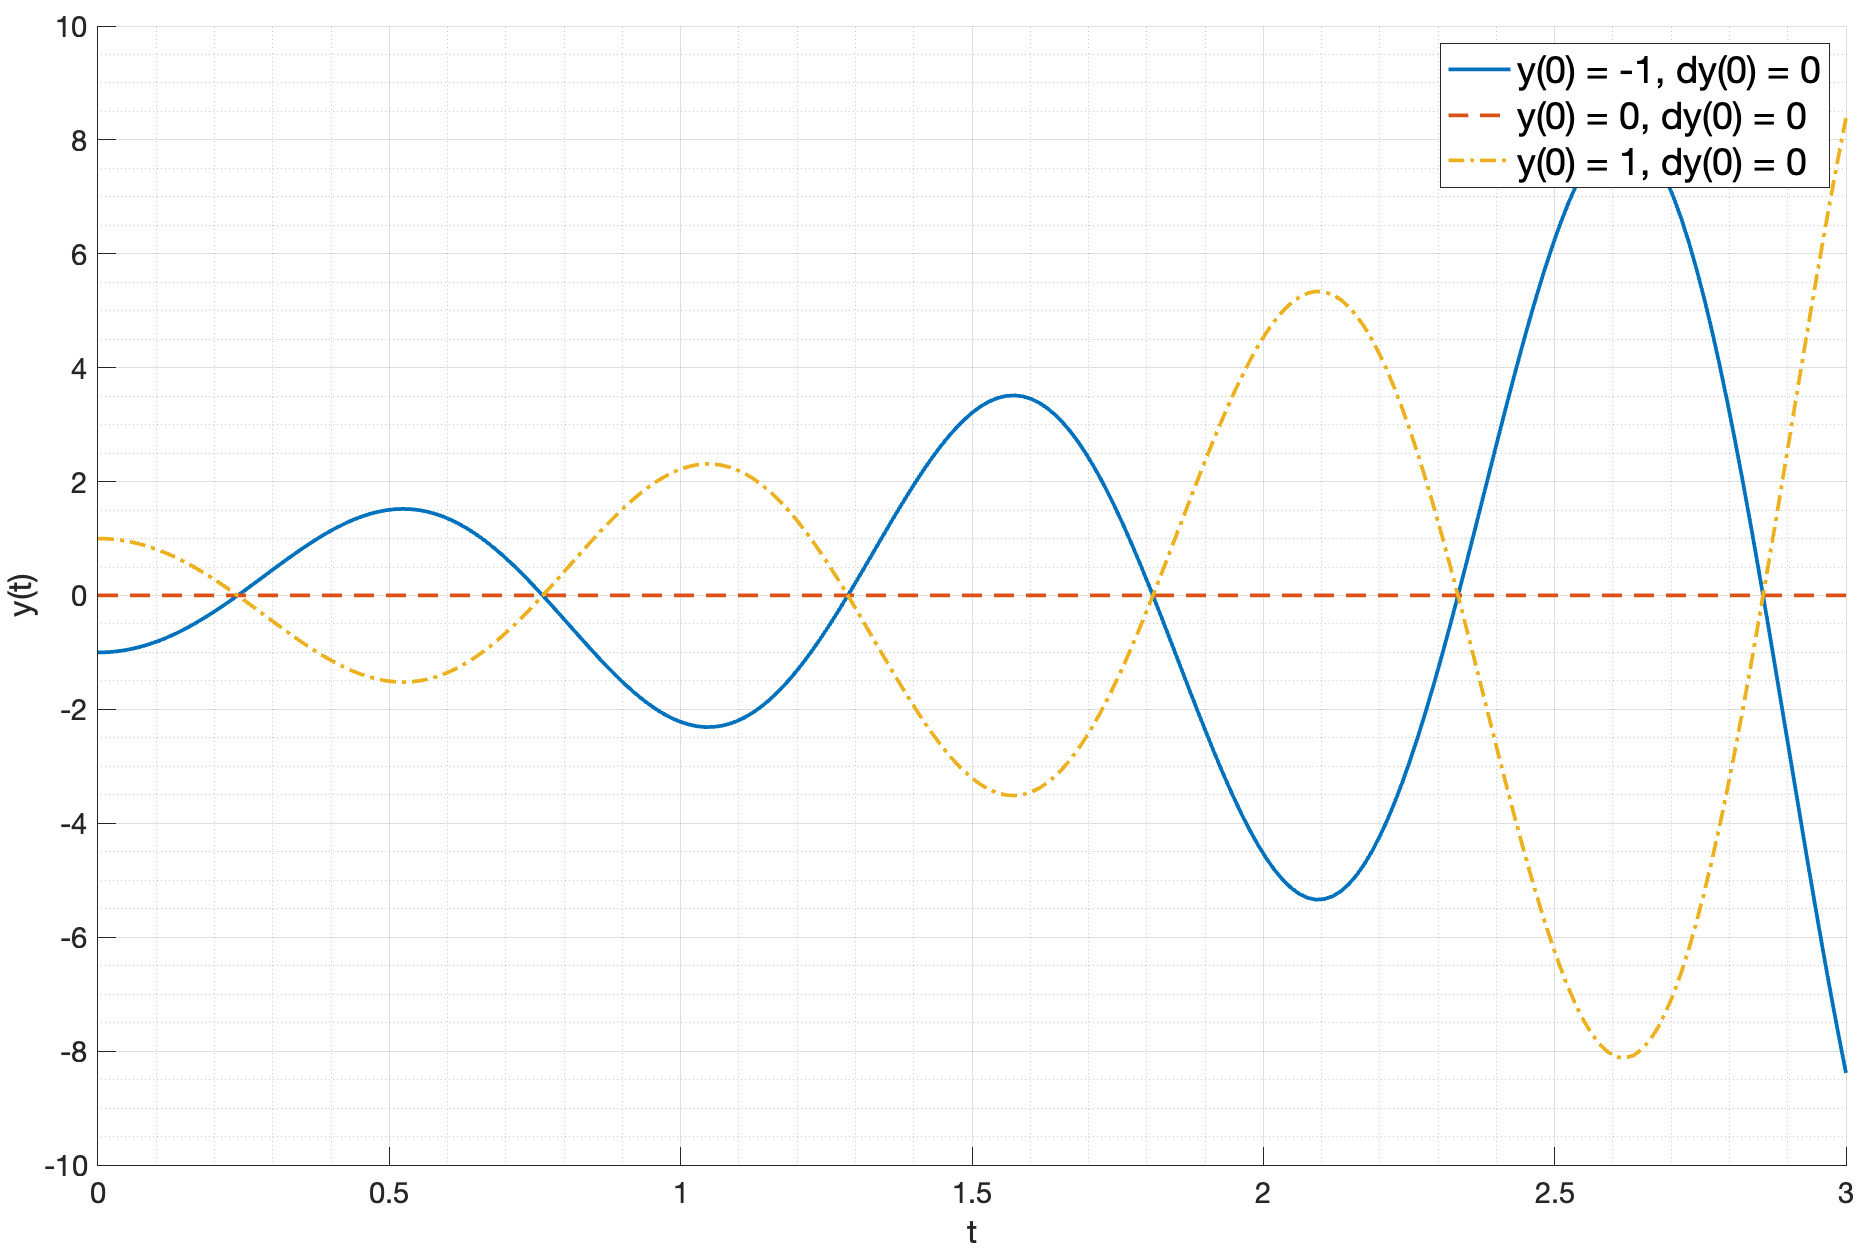
\includegraphics[width=\textwidth]{media/plots/case3_input1.png}
    \caption{$a_0 = 36.64, a_1 = -1.6, u(t) = 0.5$}
    \label{fig:case3_input1}
\end{figure}
\begin{figure}[ht!]
    \centering
    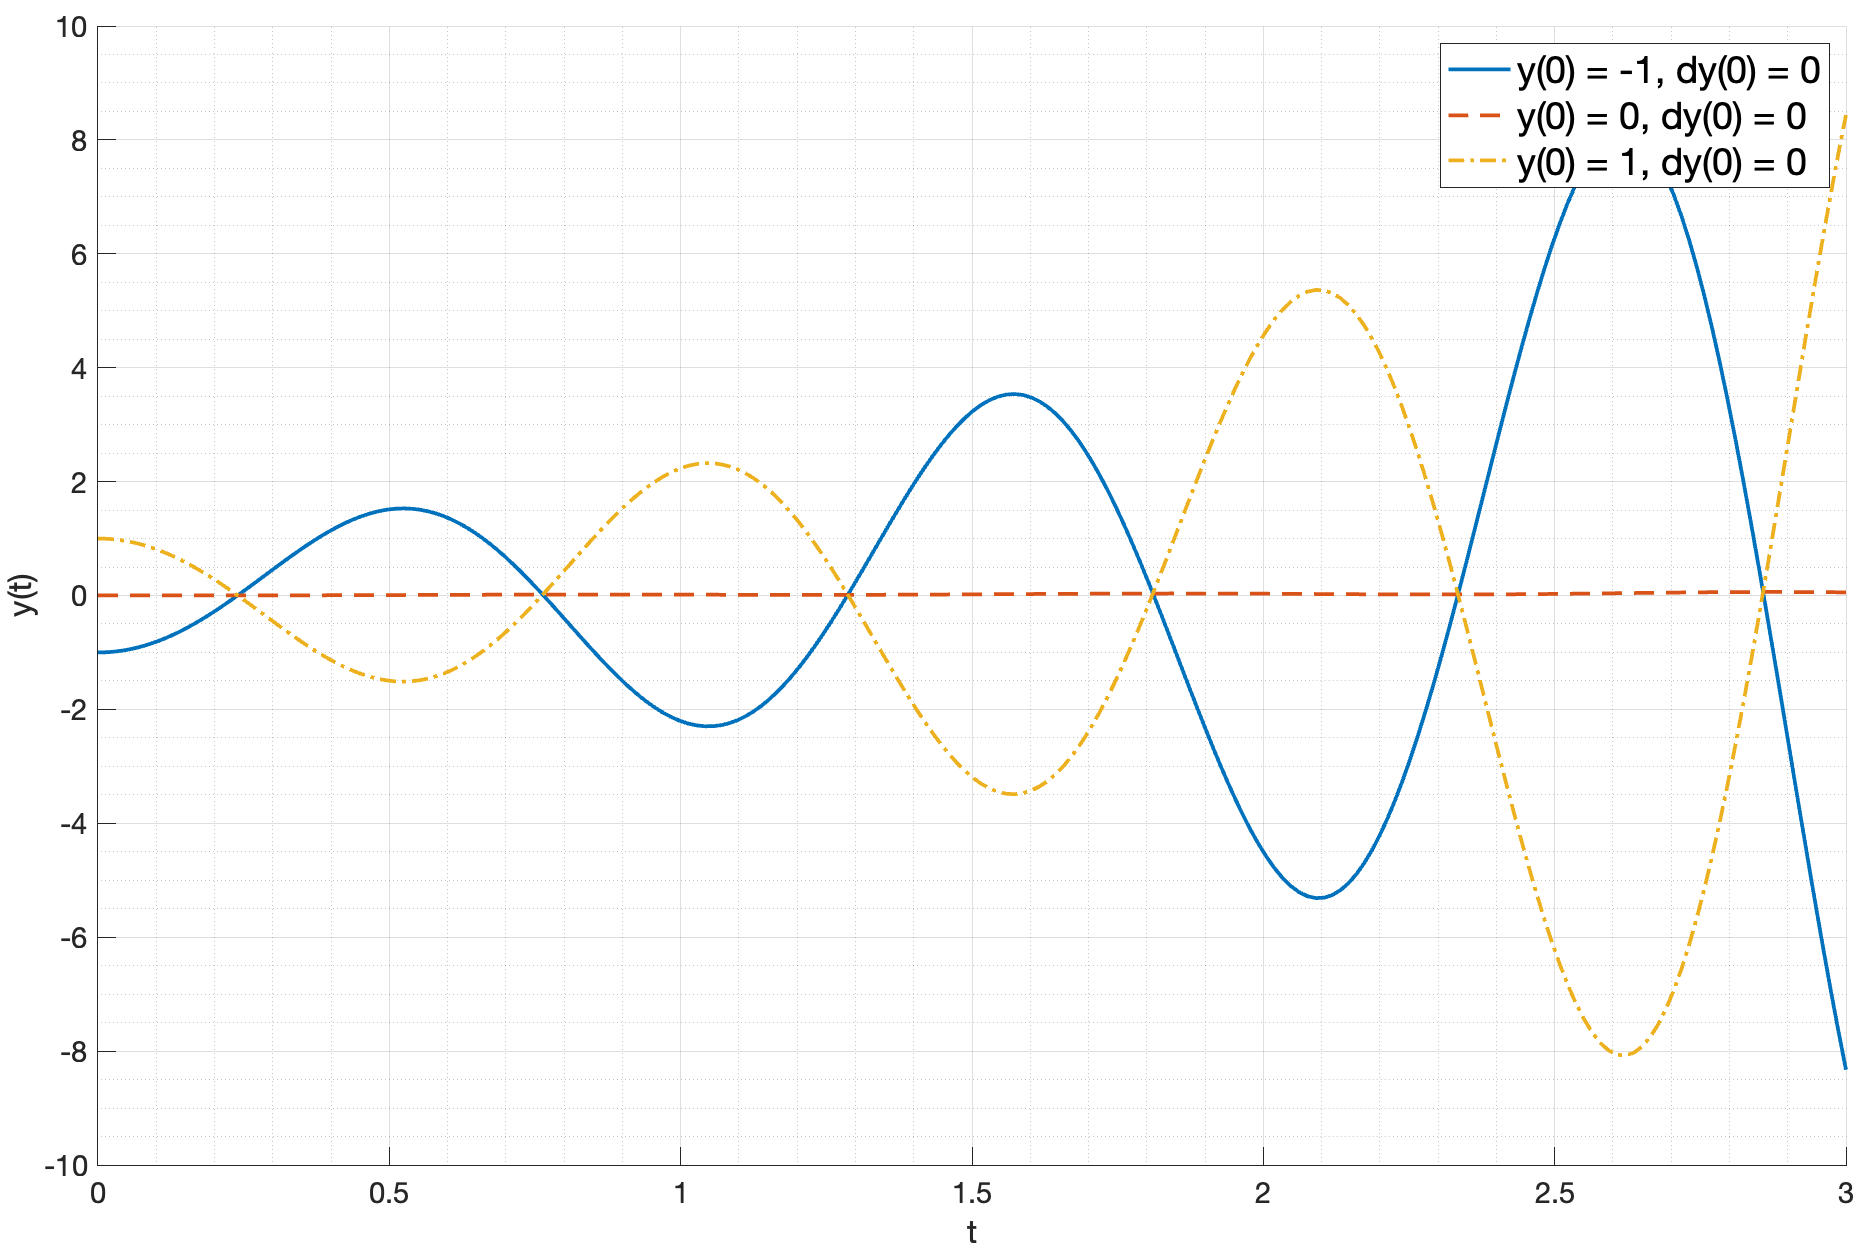
\includegraphics[width=\textwidth]{media/plots/case3_input2.png}
    \caption{$a_0 = 36.64, a_1 = -1.6, u(t) = 0.5t$}
    \label{fig:case3_input2}
\end{figure}
\begin{figure}[ht!]
    \centering
    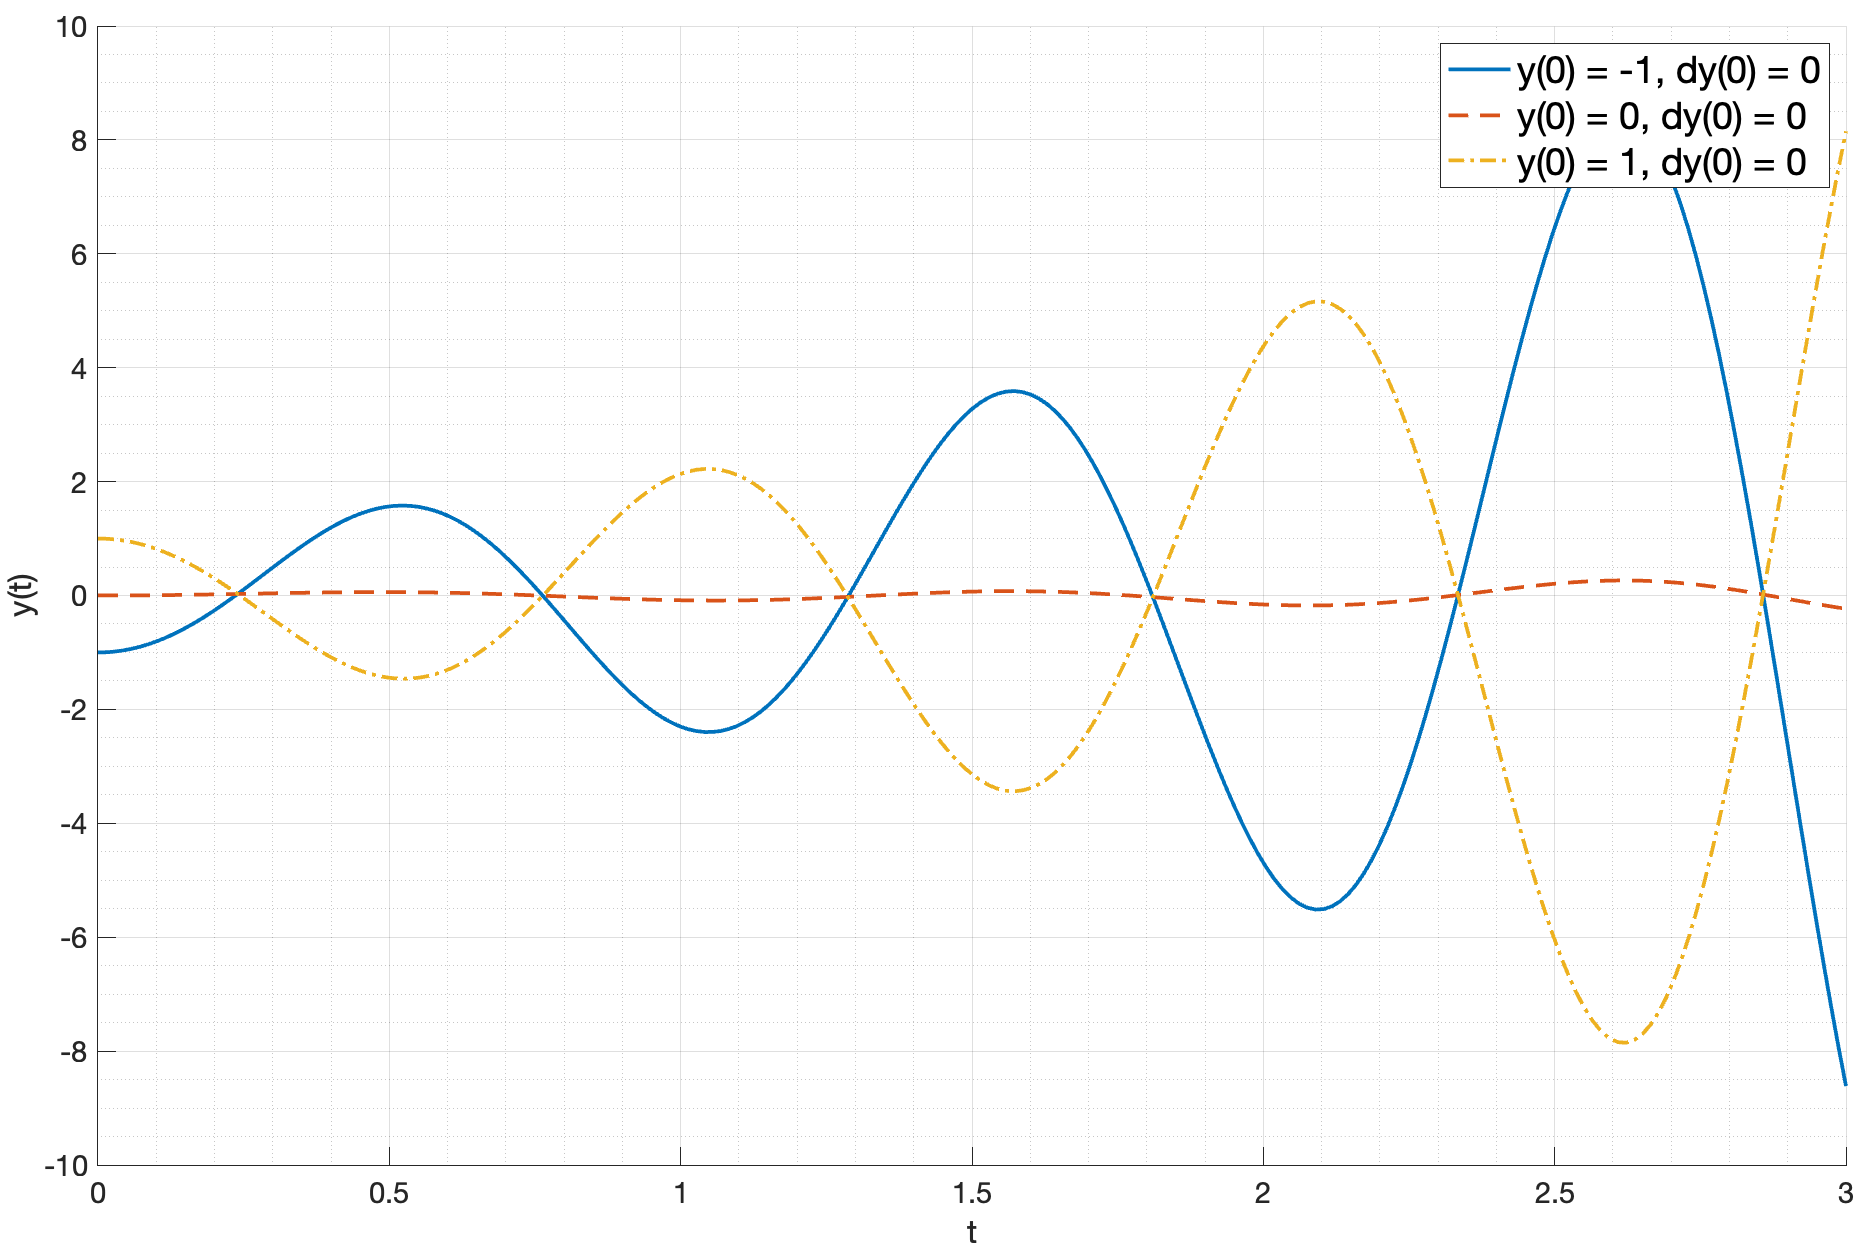
\includegraphics[width=\textwidth]{media/plots/case3_input3.png}
    \caption{$a_0 = 36.64, a_1 = -1.6, u(t) = \cos(2t)$}
    \label{fig:case_3_input_3}
\end{figure}

Посмотрим на первую систему, являющуюся устойчивой. При внешнем воздействии $u(t) = 0.5$ система приходит к установившемуся
значению, равному $0.5$. При внешнем воздействии $u(t) = 0.5t$ система не приходит к установившемуся
значению, а растет линейно. При внешнем воздействии $u(t) = \cos(2t)$ система колеблется около значения 0. 

Рассмотрим вторую систему, находящуюся на границе устойчивости. При всех рассмотренных входных 
воздействиях система колеблется около нуля, таким образом, ее стабильность не зависит от внешнего воздействия.

Рассмотрим третью систему, являющуюся неустойчивой. При всех рассмотренных входных воздействиях система 
все так же будет расти. Входное воздействие слабо влияет на поведение системы.

\subsection{Вывод}
По результатам симуляции можно сделать вывод, что внешнее воздействие влияет на поведение системы.
Даже устойчивая система может не приходить к установившемуся значению при некоторых входных воздействиях.
